\graphicspath{{Chapter2/Figs/}}

\chapter{Data collection and analysis overview}
\label{chapter2}
	
	\vspace*{\fill}\par
    \pagebreak
	 
\section{Introduction}

	The current solar observation scene has never been more ideal.
	There is currently constant space-based monitoring of the Sun but also a myriad of high-quality ground-based solar telescopes in existence.
    This is coupled with a few small space-based telescopes and sounding rocket experiments.
	Further within the next decade, the largest ground-based solar telescope will open called the Daniel K. Inouye Solar Telescope (DKIST, formerly the Advanced Technology Solar Telescope, ATST) and several highly-advanced satellites will be launched (two of which will move in to very close orbits to the Sun).
	This is an important era for solar physics going forward.
	
	Within this thesis, numerous sources of solar data were used.
	Two telescopes will be the primary focus of this chapter: the Swedish Solar Telescope (SST) and Solar Dynamics Observatory (SDO).
	While other ground-based telescopes have their data utilized here, I was able to spend 10 days at the SST and thus it gets a larger focus here.
	These two telescopes offer some of the highest quality data available to a solar physicist.
	However, all data must be processed and reduced since no telescope or instrument is perfect.
    There are always small issues with any telescope or instrument and these can cause imaging artefacts that have to be accounted for before any analysis can begin.
	Once these are taken care of, the method of analysis will need to be considered and it will vary depending on the overall aims.
	Here, the aim was to measure two properties of the observed magnetic waveguides.
    These are the cross-sectional area and total intensity through time.
    Once these two properties have been measured, deducing any periods within these signals and calculating the phase difference between them is required.
    There have been numerous methods created that aim to analyse signals and measure these properties.
    Within this thesis, three methods are employed which are the fast Fourier transform (FFT), Wavelet Transform (WT) and Empirical Mode Decomposition (EMD).  
    These methods will be discussed later in this chapter once the instrumentation is detailed.
    Finally, there is a brief analysis into the method used to measure the cross-sectional area for two example magnetic flux tubes.
	
\section{Sources of solar data}

	The work detailed within this thesis uses data from five telescopes: Swedish Solar Telescope (SST), Solar Dynamics Observatory (SDO), Dunn Solar Telescope (DST), Dutch Open Telescope (DOT) and the Swedish Solar Telescope (SVST).
    They are outlined below.
    
\subsection{Swedish Solar Telescope (SST)}

	The Swedish Solar Telescope is a one metre vacuum solar telescope located at the Roque de los Muchachos Observatory on La Palma in the Canary Islands.
	The SST was the replacement for the Swedish Vacuum Solar Telescope which used to occupy the same site and will be talked about later in this Chapter.
	The SST has a $1.1$ m lens, of which only $1$ m is usable, which is connected to a several storey vacuum tower. 
    The light collected travels down the vacuum tower into a corrector system and then to the optics bench. 
    The usage of a vacuum tower means that the collected light does not pass through any air.
    This reduces any distortion that comes from the air being heated by the beam of light.
    This improves the overall image quality. 
    The scale of the SST can be seen in Figure \ref{fig:SST}.
    It shows the building that houses the SST and the tower that contains the vacuum tower can be seen.
    
	\begin{sidewaysfigure}
        \centering
        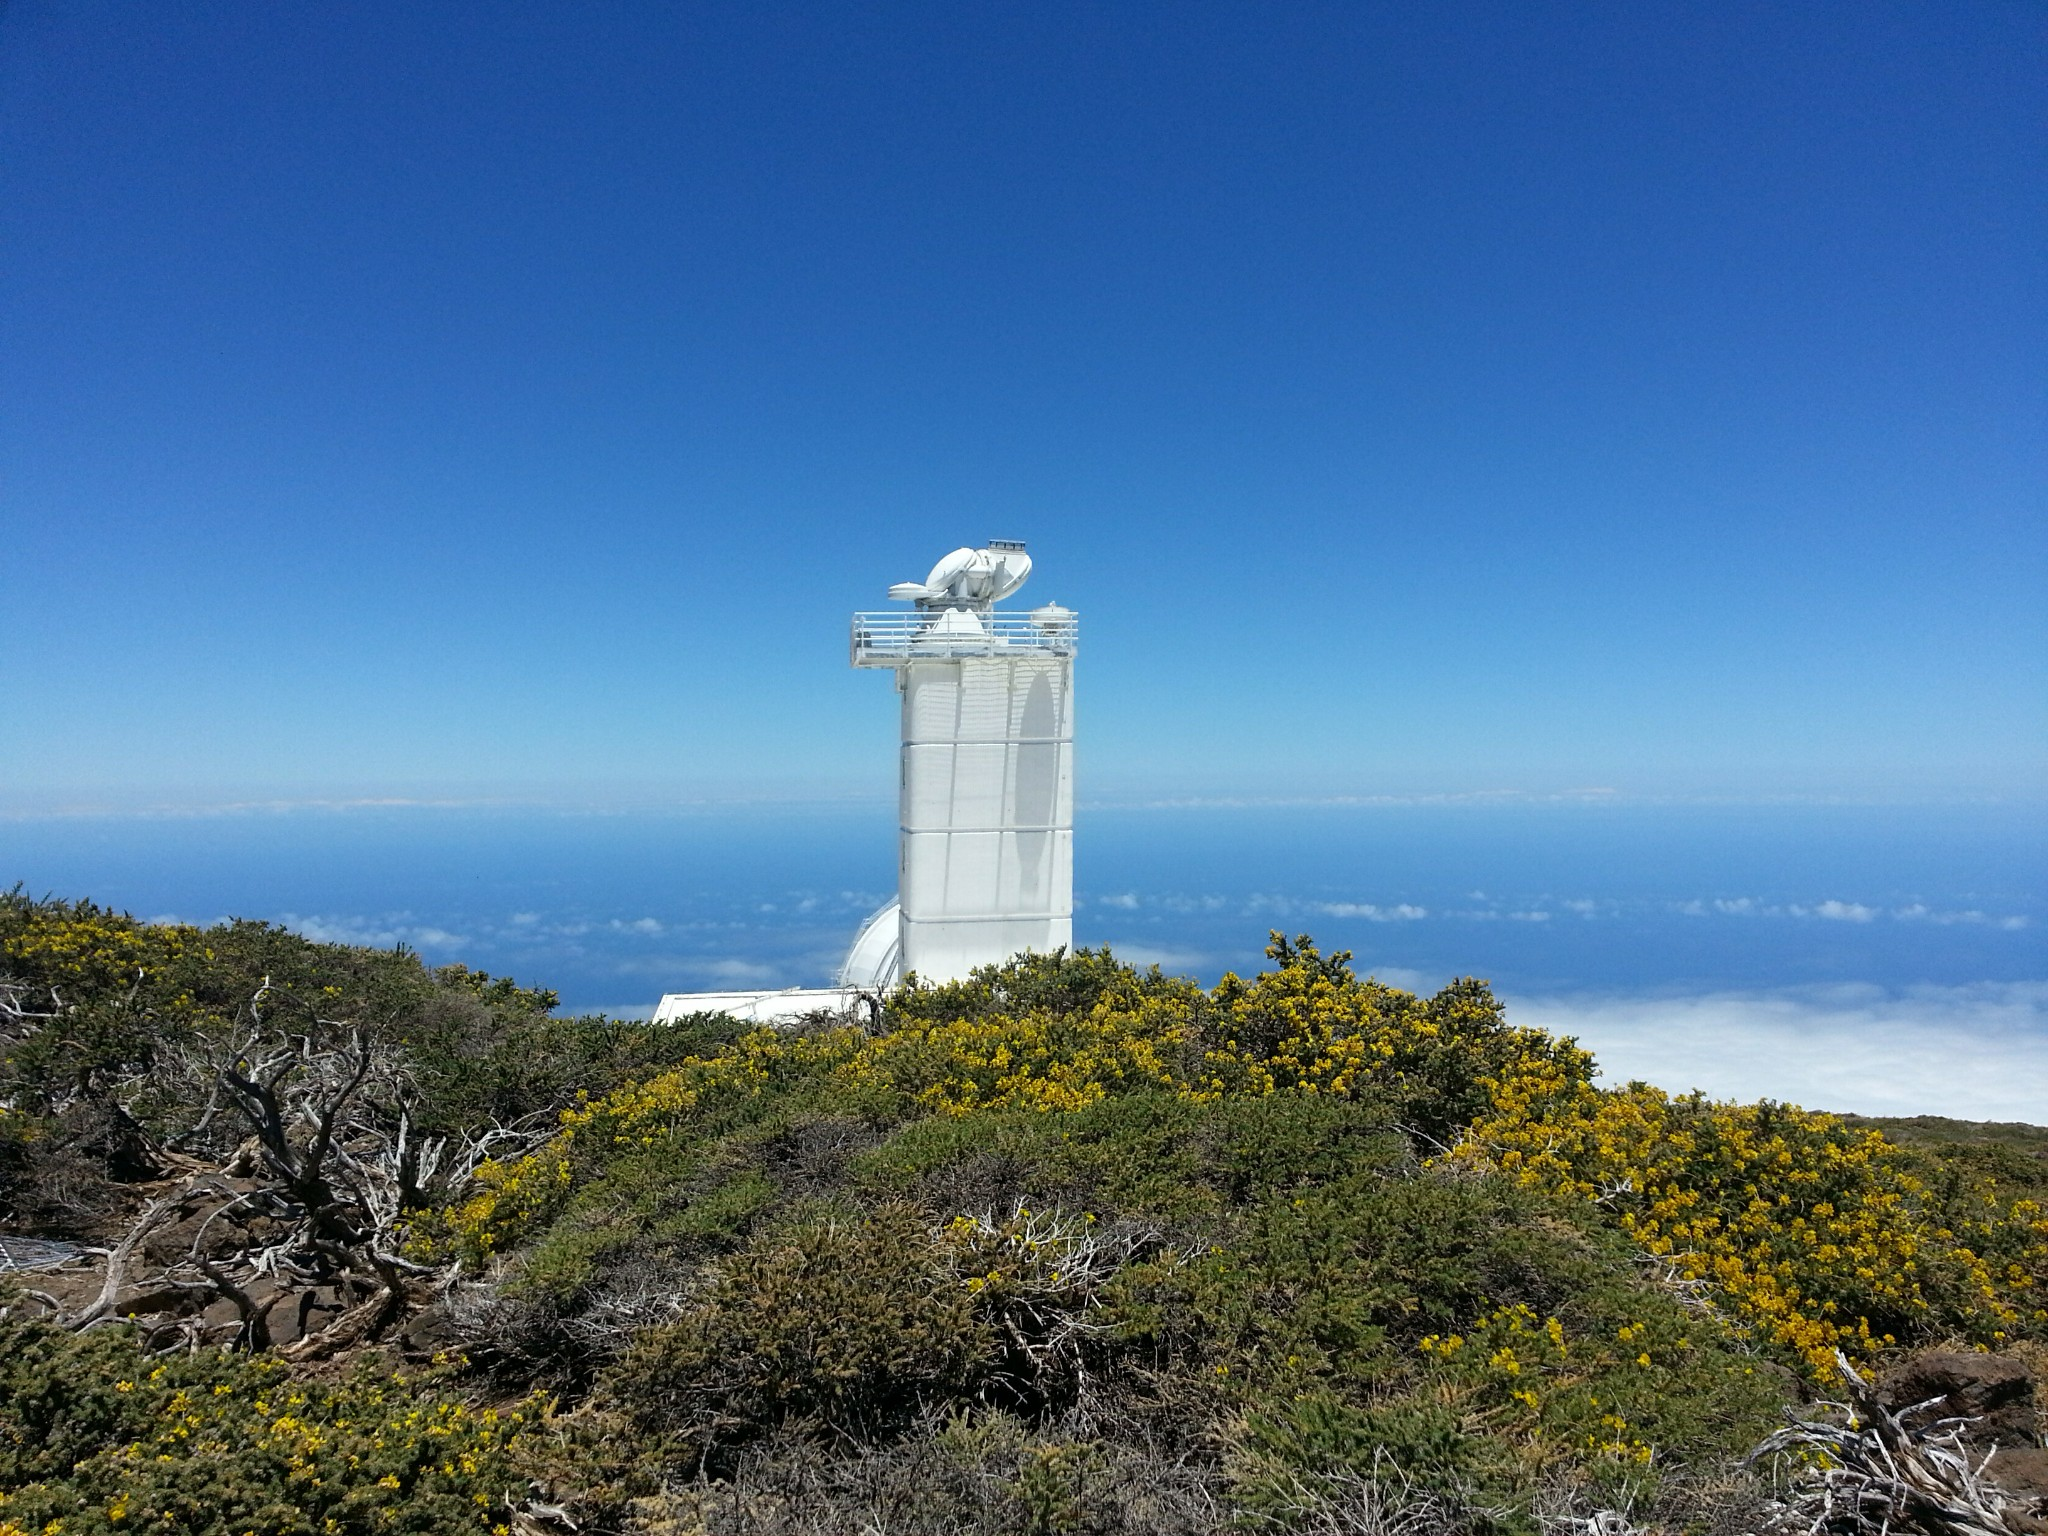
\includegraphics[width=0.75\textwidth]{SST.jpg}
        \caption{
            An image of the Swedish Solar Telescope taken from a ledge near the caldera on the island of La Palma that is part of the Canary Islands.
            The primary mirror housing can be seen at the top of the image, while the tower that conceals the vacuum tower can be seen beneath it.
            Copyright goes to the author.
           }
           \label{fig:SST}
   \end{sidewaysfigure}
         
    Further to this, the SST is equipped with an adaptive optics (AO) system. 
	AO is a term used for a process that will adjust the optics of the instrument in order to reduce the effects of turbulence from the Earth's atmosphere. 
	At a basic level, the AO at the SST has a sensor that monitors the wavefront of the incoming light wave and analyses how the wavefront is distorted. 
	This distortion is counteracted by deforming a lens, by using a voltage since the lens is made of a piezoelectric material. 
	This is not the same method used by larger and newer optical telescopes used for astrophysics that have a deformable primary mirror in conjugation with a powerful laser.
	
	The SST has two instruments, the \textit{CRisp Imaging SpectroPolarimeter} (CRISP) and the \textit{TRI-Port Polarimetric Echelle-Littrow} (TRIPPEL).
	TRIPPEL is a spectrograph with a constant diffraction grating spacing but has a shape that is similar to a sawtooth-shaped step function.
    See \cite{2011A&A...535A..14K} for a full overview of this instrument.
    
	CRISP is a tunable dual Fabry-Perot filter system.
    The wavelength range is in the red wing (510-860 nm) and the light firstly goes through a selectable pre-filter dependent on the goals of the current observational sequence.
    This allows many wavelengths to be chosen with one instrument, which is required in order to observe the height variation of the solar atmosphere.
	The Fabry-Perot is made from a pair of partly reflective mirrors that are separated by a small distance.
    By varying the distance between the two mirrors, a specific wavelength can escape the mirror system and go to the cameras.
    With the ability to vary the distance between the mirrors, the Fabry-Perot system is able to investigate the line profile, of many elements.
	Table \ref{crisp} has approximately a third of the wavelengths available with CRISP. 
	The selection of wavelengths here is the more commonly used filters that often appear in published papers.
	For example, the Fe I 630.26 nm line is used to observe the photosphere and clear granulation can be seen.
	More importantly, this wavelength is used to measure the photospheric magnetic field.
	    
	\begin{table}
         \begin{center}
         \begin{tabular}{|c|c|c|c|}
             \hline
             Pre-filter & Wavelength (nm) & FWHM (nm) & Line Core Height (km)\\
             \hline
             \ion{Mg}{} b & $517.33$ & .3 & $\le 1000$ \\
             \ion{Na}{D} & $589.7$ & .38 & $\le 500$ \\
             \ion{Fe}{I} & $630.26$ & .44 & $\le 250$ \\
             \ion{Ca}{II} k & $854.16$ & .93 & $\le 1300$ \\
             \ion{H}{$\alpha$} & $656.2$ & .49 & $\le 1500$ \\
             \hline
        \end{tabular}
        \caption{
                Summary of the more common wavelengths that are selectable with CRISP.
                Each filter has a name, wavelength at the line-core and the Full Width at Half Maximum (FWHM) and an average formation height of the line-core, which are soured from \cite{jess1}. 
                }
        \label{crisp}
        \end{center}
     \end{table}
	   
    An important wavelength is $656.3$nm and is commonly referred to as H$\alpha$.
    It is when an electron drops one energy level from the third shell to the second in a Hydrogen atom.
    This transition is the easiest method to observe the chromosphere and forms approximately $1.5$ Mm from the base of the photosphere.
    Understanding the chromosphere has become a topic of heavy interest as the ``Coronal Heating Problem'' shifted from the corona to the chromosphere over the past decade \citep{Aschwanden2007}. 
    Since the line core of H$\alpha$ samples the chromosphere, understanding how this line is formed within the solar atmosphere has become a very important topic. 
    
    However, H$\alpha$ line formation is a difficult topic.
    The line is highly complex, most likely it is dependant on numerous physical effects such as ionization or non-LTE effects. 
    Currently, the standard understanding of H$\alpha$ comes from radiative MHD simulations done, for example by \cite{Leenaarts2007} and \cite{Leenaarts2012}.
    From these  two sources, we can summarize a few properties and observations of the H$\alpha$ line core.
    
    Current research suggests that structures that appear darker, such as fibrils, in the line-core are formed higher compared to other features.
    Further, the opacity of H$\alpha$ that is formed in the upper chromosphere is temperature insensitive.
    This means that the opacity of the line is mainly determined by the mass density at these regions.
    
    The results suggest that fibrils are mainly located within magnetically dominated (i.e., low plasma-beta) regions between photospheric field concentrations of opposite polarity.
    These fibrils are aligned with the local magnetic field direction.
    Further, fibrils are located in regions where the local density is larger compared to the background chromosphere. 
    This effects the average formation height for H$\alpha$ by making it higher and thus the intensity is lower.
    Thus, fibrils can be used to trace out regions of enhanced chromospheric mass density. 
    
    Finally, the light beam at the SST is spilt into two parts when CRISP is in use.
    The red wing goes to CRISP, while the blue part goes to a series of broadband cameras.
    These wavelengths are G-band and Ca K which sample the photosphere.
    These offer some of the highest resolution images of the solar photosphere to date and are only used when the seeing is excellent. 
    Examples of the data from these cameras can be seen on the SST website (\url{http://www.solarphysics.kva.se/})
    
    One small comment on the data reduction step.
    The method used to reduce SST data is called Multi-Object Multi-Frame Blind Deconvolution (MOMFBD), which is a complex and computationally demanding method to improve the quality of the data without affecting the cadence of the observation data. 
    See \cite{Noort2005} for a full breakdown of these reduction method. 
    
\subsection{Solar Dynamics Observatory (SDO)}

	Solar Dynamics Observatory (SDO) is one of the latest space-based telescopes launched by National Aeronautics and Space Administration (NASA) \citep{2012SoPh..275...17L}.
	It can be considered as the replacement for the Solar and Heliospheric Observatory (SOHO) \citep{domingo1995soho} and the Transition Region and Coronal Explorer (TRACE) \citep{TRACE}.
    Since 2010, it has been observing the Sun constantly, beaming large quantities of data back to Earth.
	Without Earth's atmosphere in the way, it offers some of the clearest observations of the entire Sun to date. 
	The spacecraft houses three instruments: the \textit{Extreme Ultraviolet Variability Experiment} (EVE) \citep{2012SoPh..275..115W}, the \textit{Helioseismic and Magnetic Imager} (HMI) \citep{2012SoPh..275..229S} and the \textit{Atmospheric Imaging Assembly} (AIA) \citep{2012SoPh..275...17L}.
	
	EVE is designed to measure a wide range of extreme ultraviolet spectral lines with a Sun-as-a-Star method.  
	HMI measures LOS velocities as well as the LOS and vector magnetic field of the photosphere.
	AIA is a multi-wavelength instrument and is able to take images of the solar surface to the outer reaches of the solar atmosphere.
    This has offered an unprecedented view of the many layers of the solar atmosphere at the same time.
    This view can be seen in Figure \ref{fig:SDO}, which shows the full wavelength range of AIA as well as an HMI image.
    The figure showcases almost every wavelength that is available on AIA, from the low temperature lines such as $170$ nm that sample the photosphere, to the hotter lines that display the complex structure within the corona such as $13.1$ nm. 
    From HMI, there is a LOS magnetogram that showcases the magnetic field within the photosphere.
    
   	\begin{sidewaysfigure}
        \centering
        \includegraphics[width=\textwidth]{SDO.pdf}
        \caption{
                The field of view of the Solar Dynamics Observatory (SDO) satellite.
                Each image shows a different wavelength that is captured by two of the instruments on SDO, the Atmospheric Imaging Assembly (AIA) and Helioseismic and Magnetic Imager (HMI).
                The images are taken on the 17$^\mathrm{th}$ of April 2015 focusing on AR 12326.
                The columns on the side go downwards in increasing temperature response.
                The $160$ nm and $450$ nm filter of AIA is missing from the image.
                }
        \label{fig:SDO}
    \end{sidewaysfigure}
    
\subsection{Other ground telescopes}

	Data from three other ground-based telescopes is used within this thesis.
	What follows is a brief summary of each one and more details are given within the chapters where the data from these telescopes are used.
    
	First, the Swedish Vacuum Solar Telescope (SVST) which was the predecessor to the current SST.
	It had a 47.5 cm mirror with several wavelength narrowband filters with no AO.
    The narrowband filters were not too dissimilar to the wavelengths in Table. \ref{crisp}.
    See \cite{1991AdSpR..11..129S} for a full overview of the SVST.

	Second, the Dutch Open Telescope (DOT) is an open-air solar telescope that is now retired. 
	The DOT is located next to the SST on La Palma.
    It has a very compact design that is quite different to the SST.
    It has a mirror that is slightly smaller than the previous SVST, at only 45 cm.
    The full instrumental setup consisted of 6 cameras each with a different narrow band filter.
	With no AO, it used a more unconventional method to lessen seeing effects.
	The telescope was on a mount several meters high, which was open to the atmosphere.
    As such, the strong winds blew across the mirror reducing seeing effects from temperature gradients that are caused by the ground, which reduced image distortion.
    Further, it used high frequency cameras that allowed speckle reconstruction.
    Speckle reconstruction is a method to reducing the effect of Earth's atmosphere on the images obtained.
    But using high-speed camera able to capture many frames in one second, the frames are combined in order to form a model of the distortion from the atmosphere. 
    This effect however, reducing the cadence of the observation.
    See \cite{rutten} for a full overview of the DOT.
    
	Finally, the Richard B. Dunn Solar Telescope, located at Sacramento Peak in New Mexico and is run by the National Solar Observatory (NSO).
    It has a 76 cm mirror and is a vacuum telescope similar to the SST but its design is unique.
    The tower itself moves, unlike the SST where it is just the telescope mount, it seated on a ring of liquid mercury and it allows it to rotate to track the Sun throughout the day. 
    It has many instruments but the focus here is on two of them: \textit{Rapid Oscillations in the Solar Atmosphere} (ROSA) and \textit{Interferometric Bidimensional Spectrometer} (IBIS).
    ROSA is a synchronised 6 camera system similar in principle to the system on the DOT. 
    It captures images at high frequency rates and uses narrowband wavelength filters that sample the photosphere and chromosphere.
    Much like the DOT, it uses speckle reconstruction to improve the quality of the images, while IBIS is similar to CRISP at the SST.
    It consists of two Fabry-Perot interferometers that operates in the red wing (550-860 nm) and allows in-depth line scans for specific wavelengths as well as measuring polarized light in spectropolarimetric mode.
    See \cite{jess1} and \cite{cavallini2006ibis} for a full overview of ROSA and IBIS respectively.
       
\section{Signal analysis}

	Once the process of data acquisition is finished and the data has been reduced using methods that are specific for that telescope or instrument, analysis of the data can begin.
    The method used will vary depending on the overall science goal or aim.
    For example, statistical studies require crunching through large quantities of data in order to categorize the general properties of the phenomenon that is under investigation. 
	Other studies will focus on single events, either due to the lack of a large selection of data or if the event under investigation is rare.
	The analysis undertaken within this thesis is focused on measuring the properties of waves in several sunspots and magnetic pores and later a single dataset studying RPWs.
   	
	From Chapter 1, it is clear that to observe MHD sausage waves in cylindrical structures, the phase relations between specific observational quantities such as the cross-sectional area and total intensity are required.
    While further phase relations are available, the two quantities used were the ones only possible with the ground-based data available at the time.
    As a result, the focus has been on the cross-sectional area and total intensity perturbations. 
    Once these signals have been measured from the datasets used, the periods and phase difference of these signals must be found.
    The methods used are the Fast Fourier Transform (FFT), wavelets and Empirical Mode Decomposition (EMD) and are discussed below.
     
\subsection{Fast Fourier Transform (FFT)}

	The first method is the Fast Fourier Transform (FFT).
	Its name is a reference to the fact that the FFT is very fast computational algorithm of the Discrete Fourier Transform (DFT).
    It was first introduced by \cite{cooley1965algorithm}.
	The Fourier Transform is a mathematical method to decompose a signal which is assumed to be periodic into its constituent frequencies.
	Generally, it is common to have a real-valued signal input into the FFT and the resulting output is a complex number.
	The absolute value of this output is the amount (or power if squared) of each frequency in the original signal and the complex part is the phase shift of the sinusoidal function at that frequency.
    
    An example of this can be seen in Figure \ref{fig:signal_overview}.
    The top left image is of an artificial signal, of the form, $$\sin\left(2\pi \frac{x}{5}\right) + \cos\left(2\pi \frac{x}{10}\right) + 5\times\mathrm{random\ noise},$$ where the noise is Gaussian distributed.
    The top right image is the output after this signal is passed into the FFT.
    It is a power spectrum, where we have power as a function of frequency.
    The two peaks that can be seen correspond to the two frequencies of the artificial signal.
    The small peaks that are littered in the power spectrum correspond to the uniform noise that was added to the signal.
    
   	\begin{sidewaysfigure}
           \centering
           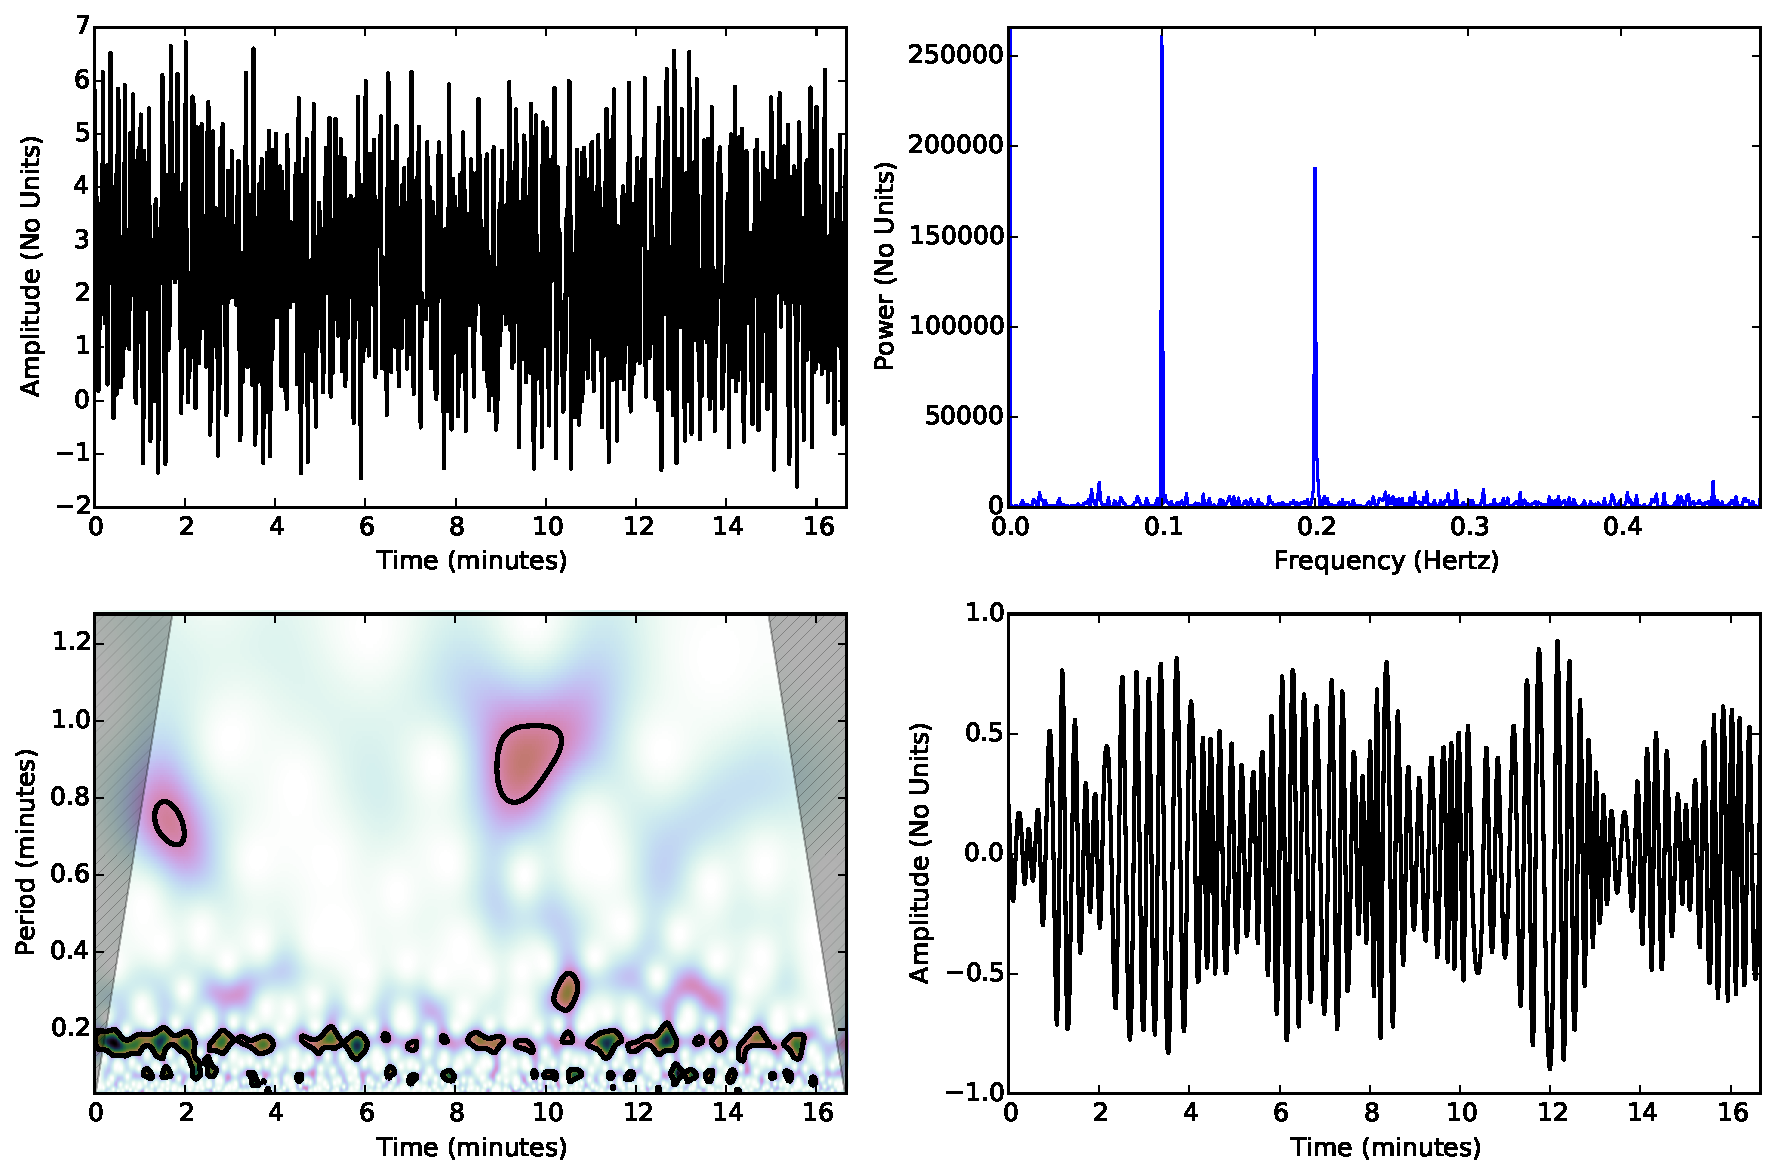
\includegraphics[width=0.85\textwidth]{signal_overview.pdf}
           \caption{
                   An example of the signal analysis methods used in this thesis. 
                   The upper left plot is of an artificial signal with noise.
                   The upper right plot is a power spectrum from the FFT.
                   The largest two peaks shows the frequencies within the artificial signal.
                   The bottom left plot is a wavelet power spectrum.
                   It expands on the FFT by offering a 2D view of the frequency spectrum with time.
                   So it is possible to see what period is within the signal but also at what time it is located at and its duration.
                   The bottom right plot shows an IMF output from a EMD algorithm.
                   The IMF contains one of the periods from the artificial signal used and this corresponds to the smaller frequency within the artificial signal.
                   }
              \label{fig:signal_overview}
     \end{sidewaysfigure}
	
	The nature of signal analysis means that each individual method has both positives and negatives.
	Generally, the type of signal or the overall aim will determine the method used.
	To start, input signals have a finite length which is the case for the Fourier Transform. 
	This fact means that artefacts are introduced as a result, however, this is not unique to the FFT and most signal analysis algorithms suffer from this issue. 
	The FFT has an effect known as frequency leakage.
    It is where, if the input signal is non-periodic or the input signal has no closed form transform, there is smearing in the frequency spectrum.
    This means that the power is not confined to the correct frequency and spreads, so other frequencies close to the strongest frequencies will be masked if the difference in power between two frequencies is large.
	This can be overcome by using a window function on the original signal which alters the outcome of the FFT in order to reduce these effects.	
    Finally, another important part of the FFT is the output can be reversed.
    It is possible to recover the original signal using the Inverse FFT (IFFT).
    This fact means that one can create a frequency window and apply it to the frequency spectrum.
    This can be used to filter parts of the frequency spectrum that contain information that is unnecessary or return a new signal to see the behaviour at specific frequencies.
    It is commonly used method in signal analysis and is used within Chapter 5.
    	
\subsection{Wavelet transform}

	The second method employed is called the Wavelet Transform.
	A wavelet is a function that is constrained in time and frequency space i.e., localised within these specific domains.
	The base function used is called the mother wavelet and variations of this function are called daughters.
	This factor is important, as the FFT will, when given a 1D signal, output a 1D frequency spectrum.
	The wavelet algorithm will return a 2D spectrum where the extra dimension is time.
	This means you can also know what frequency is within the signal but also at what time in the signal that frequency exists and for how long.
	This is a more powerful method due to this fact, but also, each mother wavelet have different properties, so depending on the goal of the signal analysis, by changing the mother wavelet, different information can be extracted. 
	For example, the wavelet chosen within this thesis is the Morlet Wavelet.
	It is defined as,
	\begin{equation}
		\Psi_0(\eta) = \pi^{-1/4} \exp(iw_0\eta)\exp(-\eta^2/2).
	\end{equation}
    which can be summarized as a plane wave modulated by a Gaussian.
	It has good frequency resolution but it comes at a cost of its time resolution, while another wavelet called the Paul wavelet has a poorer frequency resolution but it has an increased time resolution.
	This allows the method to be highly variable.
    
    The top right image of Figure \ref{fig:signal_overview} shows the output of a wavelet algorithm on the artificial signal.
    The dark regions show an increase in the power, which shows where the periods of the signal are.
    The wavelet algorithm has the ability to calculate the significance of any regions of power and the black contour lines show this.
    The contour lines shown are for 95\% significance. 
    Further, much like the FFT, the finite length of a signal creates edge effects for the wavelet.
    This can be seen as the cross-hatched regions, these mark the region where the finite length of the signal affects the wavelet transform.
    The hatching properties are different for each mother wavelet.
    
    Finally, the wavelet transform allows for direct comparison of two signals.
    It is possible to calculate the cross-wavelet of two signals as well as correlation and the phase difference using the wavelet transform.
    This fact allows the wavelet transform to be used to measure the phase difference of the cross-sectional area and total intensity signals, which is the main method used to find the phase difference within this thesis.
    See \cite{WAUO} for an overview of the wavelet transform and its applications.
    
\subsection{Empirical Mode Decomposition (EMD)}

	Finally, we have Empirical Mode Decomposition (EMD).
	As the name suggests, this method is not based off a mathematical theorem or transformation.
    The algorithm will output several signals, the residual and Intrinsic Mode Functions (IMFs).
    The residual is the left over signal from the algorithm and tends to contain any slow varying background trend.
    An IMF will generally be a simple oscillatory mode, ideally it should be only one of the frequencies within the original signal.
    There are two requirements in order to be considered as an IMF.
    Firstly, the number of extrema and zero crossings must either be equal or differ by one.
    Secondly, the mean value of the envelope defined by the local maxima and the envelope defined by the local minima equals zero.
    
    The steps of the algorithm are as follows.
    \begin{enumerate}
        \item The minima and maxima of the input signal are found.
        \item A spline fit of the minima and maxima points is computed.
        \item The resulting minima and maxima curves create an envelope that encompass the signal.
        \item This envelope is subtracted from the input signal and this process is repeated again until a specific criterion is met. This is termed sifting.
        \item The resulting signal is called an IMF and is subtracted from the original signal. The leftover signal is termed the residual.
        \item This process repeats itself again on the residual signal until a set number of IMFs are obtained leaving nothing but the final residual signal.
    \end{enumerate}
    There are two comments to be made here.
    Firstly, the stopping criterion for the sifting varies and there are two common ones.
    The first one is, if the standard deviation of the sifted signals is lower than a given limit, the process stops.
    The second one is called the S number which, if the same signal is returned by the sifting process more than S times, causes the process to stop.
    Secondly, the overall algorithm has no method of deciding when enough IMFs have been found, so the number picked is arbitrary, but generally the algorithm will stop before this limit is reached.
    As the residual becomes linear with each IMF removal, the fitting algorithm will stop naturally since there are no more extrema points.
    The resulting set of IMFs, contain the periods within the original signal, while the residual should contain any background trend.
    Much like the FFT, you can reverse the method as the sum of all of the IMFs and residual will return the original input signal.

    The EMD allows, much like the cross wavelet, the ability to find the phase difference between two signals containing the same periods.
    With a direct comparison of the IMFs of one signal to another, you can measure the phase difference between them.
    For example, this was carried out by \cite{morton2011}.
    The EMD algorithm is also very good at separating noise from a signal, which is what the first IMF generally contains.
   
    The drawbacks for the EMD are most focused on the method, since it has no mathematical foundation like the FFT or wavelet.
    The most important issue for the EMD is the spline fit that creates the envelopes.
    The envelope fit with each iteration, starts to become very large at the edges since there is nothing to constrain it.
    As such, when these are subtracted from the signal, the resulting IMFs display large swings at the start and end, so these edge effects will easily affect the output.
    To counter-act this effect, several methods have been suggested to lessen this issue and it will generally involve adding extra extrema points on both sides to constrict the spline fit.
    See \cite{huang} or \cite{terradas} for an overview of this method.
    
\section{Area analysis}

	The core work presented in this thesis is analysing the cross-sectional area of magnetic pores and sunspots.
	So it is important to be able to confidently measure the cross-sectional area.
    The base idea is to contour the structure and use that as a measure of its cross-sectional area.
    The issue is how various methods have been used in published research.
    While many never state exactly how they contoured a sunspot or a magnetic pore.
	\cite{morton2011} used a $2.5\sigma$ threshold of the mean background intensity for G-band data.
    Sigma (or $\sigma$) refers to the standard deviation of the background intensity.
	More recently, \cite{0004-637X-806-1-132} used $2.2\sigma$ of the mean background intensity for their data.
    This was to account for the change in contrast between several different wavelength filters.
    Since their aim was to measure the cross-sectional area of a pore from the photosphere to the lower chromosphere.
	
	What will occur here, is an analysis on what effect changing the value of sigma has on the resultant cross-sectional area signal.
    The value of sigma can appear to be arbitrary and there is an assumption that the intensity of the background photosphere is a normal distribution and as such sigma can be used to contour these magnetic structures.
    To be more precise, whether different sigma values will give different periods after signal analysis or if the value of sigma once set within a certain range does not change the output is of interest, especially since the current selection of ground-based solar telescopes have resolutions similar to each other and this could be the limiting factor in detecting these oscillations.
    
	This analysis is only for ground-based data and for elemental lines that sample the photosphere directly.
	The chromosphere lines used traditionally (\ion{Ca}{II} and H$\alpha$ line core) make resolving the fine boundaries of a sunspot or a magnetic pore very difficult.
    This is an area for future investigation.
    
    \subsection{Data}
    
    The data for this investigation comes from two instruments on the DST: IBIS and ROSA.
    
    The IBIS dataset consists of an image series of a H$\alpha$ line scan.
    The DST was centred on a sunspot in AR 11579.
    The observation run was on the 30$^{\mathrm{th}}$ of September 2012 at 15:00 UT until 15:16 UT with a cadence of 6.8 seconds.
    The full field of view (FOV) was 96\arcsecs by 96\arcsecs with a pixel size of 0.097\arcsecs.
    The part of the line scan used here is -0.7 nm, which falls into the blue wing of the H$\alpha$ line profile.
    This part of the line profile samples the photosphere strongly and will show Ellerman Bombs as well as Type II spicules.
    See \cite{2013A&A...560A..31N} on the reduction methods for this IBIS data.

    The ROSA dataset consists of an image series of G-band narrowband filter images.
    The DST was centred on a small magnetic pore cluster in AR 11683.
    The observation run was on the 6$^{\mathrm{th}}$ of March 2013 at 19:27 UT till 20:02 UT with a cadence of 2.11 seconds.
    The full FOV was 115\arcsecs by 115\arcsecs with a pixel size of 0.12\arcsecs.
    The narrowband filter means that only the line core was sampled and this corresponds to the low photosphere for G-band.
    See \cite{0004-637X-806-1-132} for the reduction methods for this ROSA data.
    
    Both magnetic structures can be seen in Figure \ref{fig:data_overview}.
    The image on the left showcases the  IBIS sunspot while on the right, the ROSA pore is displayed.
    Both images are context images and do not show the full FOV of each instrument during that observation run.
    Both structures are stable throughout their respective observation run.

    \begin{sidewaysfigure}
        \centering
        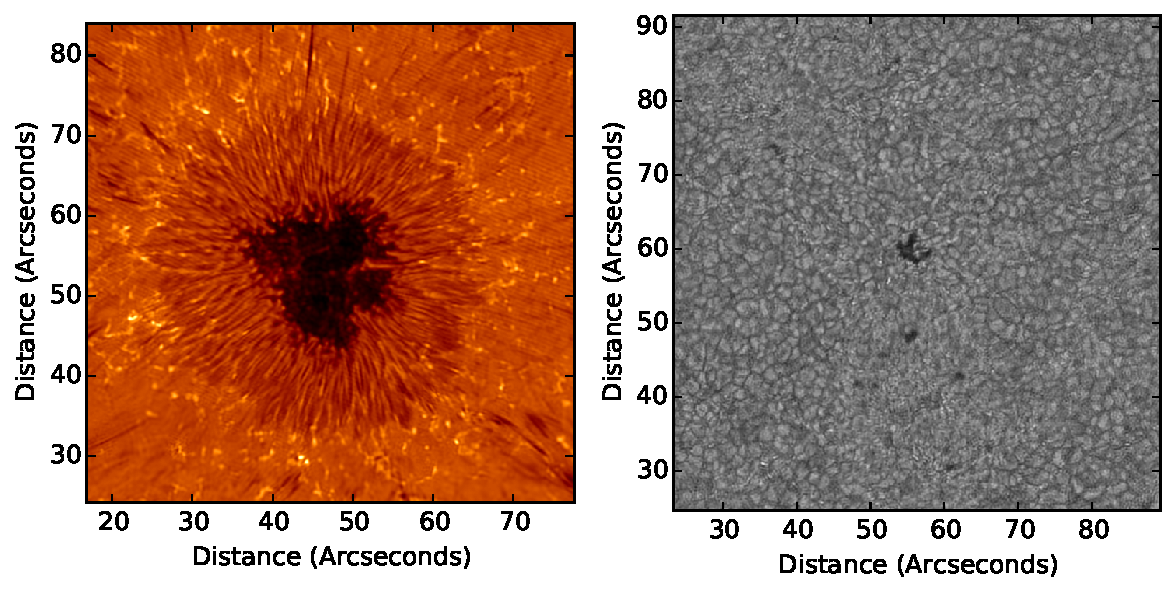
\includegraphics[width=\textwidth]{overview.pdf}
        \caption{
                The left figure is the cropped field of view (FOV) for IBIS.
                It is in the blue wing of the H$\alpha$ line profile which samples the photosphere and not the chromosphere that the line core samples.
                The sunspot is in AR 11579 and was taken on the 30$^{\mathrm{th}}$ of September 2012 at 15:00 UT until 15:16 UT.
                The right figure is of a cropped FOV for ROSA.
                It is the G-band narrowband filter which samples the lower photosphere.
                The focus is on a small magnetic pore cluster, in AR 11683 and was taken on the 6$^{\mathrm{th}}$ of March 2013 at 19:27 UT till 20:02 UT.
                The magnetic pore investigated here is the larger one at the top.
                }
        \label{fig:data_overview}
    \end{sidewaysfigure}
        
    The method used to contour these structures is as follows.
    The starting point is to find a large area of quiet-Sun photosphere, where there is no strong magnetic features.
    This area is used to calculate the mean intensity and a histogram of this area should form an approximate normal distribution.
    The normal distribution means that the standard deviation ($\sigma$) can be used to select specific pixels within the image.
    As the number of standard deviations is increased, more of the data will be covered by the distribution;
    By limiting the pixels of interest by having a limit that is lower than say two standard deviations or higher, the pixels left over will be the darkest 5\% of pixels, or the other way round would return the brightest 5\% of pixels.
    Theoretically, the lower limit should return the pixels for sunspots and magnetic pores which are substantially darker than other features in the photosphere.
    By counting these pixels, this should correspond to the cross-sectional area of these magnetic structures.
    
    Figure \ref{fig:method_overview} shows this method applied on the example datasets.
    The left column shows the two context images of these datasets shown in Figure \ref{fig:data_overview}.
    However, added to these images are four contours coloured as follows: blue, green, purple and orange.
    Each colour represents a different multiplier for the standard deviation.
    The sunspot and magnetic pore do not share the same range of multipliers.
    For the sunspot the multipliers are 3, 3.5, 4, 4.5 and for the pore they are 2, 2.5, 3, 3.5.

    \begin{sidewaysfigure}
        \centering
        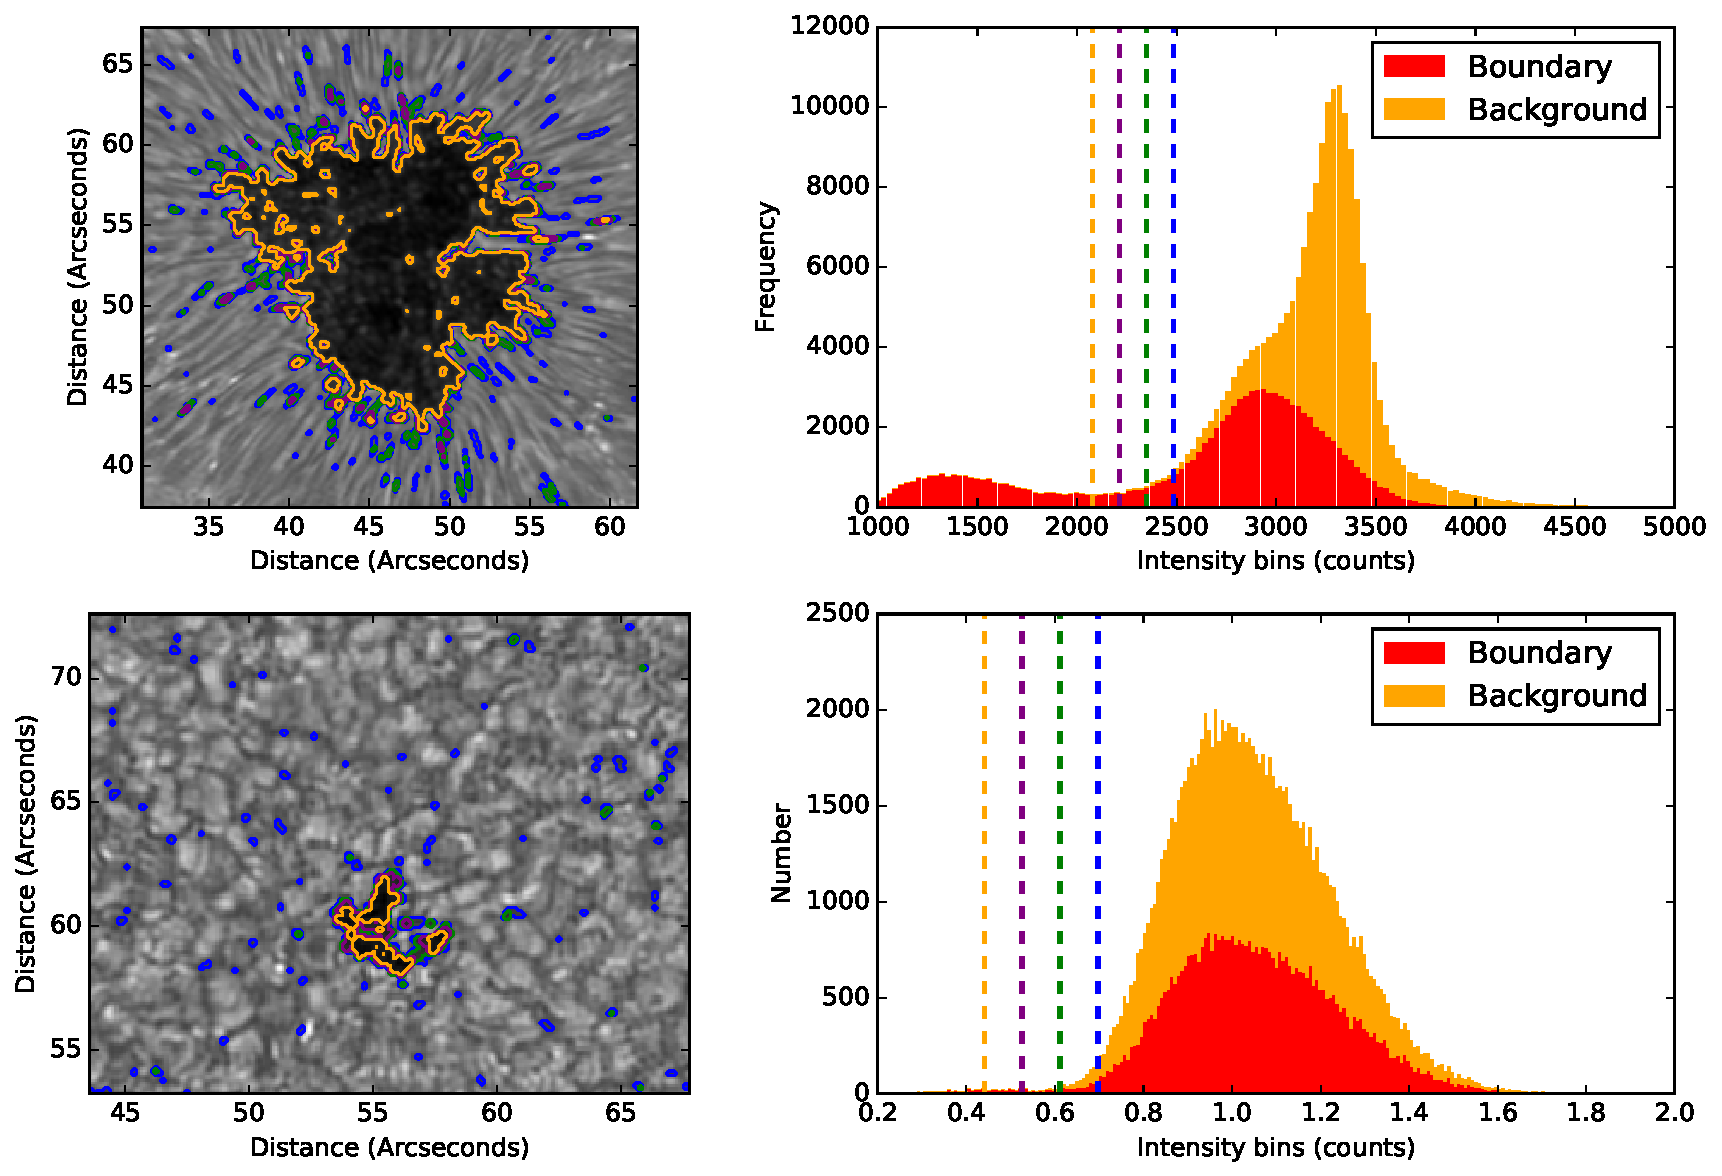
\includegraphics[width=0.85\textwidth]{method_overview.pdf}
        \caption{
                An overview of the method used to contour the magnetic structures in this thesis.
                The left column shows context images of the datasets shown in Figure \ref{fig:data_overview}.
                They have the contours of the various sigma multipliers shown.
                The contour colours of blue, green, purple and orange correspond to 3, 3.5, 4 and 4.5$\sigma$ and 2, 2.5, 3 and 3.5$\sigma$ for the sunspot and magnetic pore respectively.
                The right column shows histograms of the background photosphere in yellow and of the context image of the magnetic structures shown on the left in red.
                The vertical lines shown display where the $\sigma$ values end up on the histogram.
                These are coloured in the same vein as the left column contours.
                }
        \label{fig:method_overview}
    \end{sidewaysfigure}
    
    Firstly, the sunspot observed with IBIS will be investigated.
    The contouring for the sunspot at the lower sigma multipliers does capture small parts of the penumbra.
    For example at 2.5$\sigma$ (which is not shown), the contour was the entire sunspot, i.e., the umbra and penumbra.
    The jump to 3$\sigma$ (blue) curtails most of the penumbra.
    Once sigma is at 3.5 and 4, which correspond to the green and purple contours, the penumbra that is contoured has shrunk nearly to zero.
    However, it is not until we reach the largest sigma value (4.5) that the penumbral area disappears completely.
    The reason for this can be seen in the right column of Figure \ref{fig:method_overview}.
    The top figure is of a histogram of both the background which is in yellow and the context image on the left which is in red.
    The background here is not in a normal distribution and the reason for this is that the full FOV does not have a good area of quiet-Sun photosphere.
    The wings of H$\alpha$ show a variety of features, including Ellerman Bombs and Type II spicules, so finding an isolated region becomes harder.
    Further, the full FOV is more limited in IBIS than ROSA or CRISP. 
    This means that the sigma value is skewed and thus the multiplier will have to be higher to counter act this.
    Finally, the sunspot histogram shows a clear difference between the penumbra and umbra.
    The histogram can be split into two parts, the left part contains the umbra and the right part contains the penumbra.
    The penumbra for this sunspot occupies a larger portion of the context image which explains why the right part of the histogram is taller.
    At the intensity values between 1800 to 2300, the histogram plateaus and within this region is where the range of sigma multipliers lie. 
    The vertical coloured lines correspond to the same colour contour lines in the context image.
    It is possible to claim that, as long as the sigma multiplier is between this range, we have isolated the penumbra from the umbra.
    Using this as guide, it makes it easy to show that the sigma multiplier of 4.5 would be an ideal value since it gives the values in the middle of the plateau.
        
    Secondly, the magnetic pore observed with ROSA will be investigated.
    The overall picture is quite different and the main reason for this is the lack of a penumbra.
    While there was a plateau that separated the penumbra and umbra for the sunspot, this is missing for the magnetic pore and the sigma multiplier is harder to directly choose.
    The sigma multipliers are lower for the magnetic pore and are 2, 2.5, 3 and 3.5.
    Each of these are shown on the bottom left image of Figure \ref{fig:method_overview}.
    These values again correspond to blue, green, purple and orange.
    The lowest multiplier contours large amounts of the background photosphere.
    However, all the larger multipliers contour only the magnetic pore.
    There are clear parts of the magnetic pore that are ignored with these higher multipliers.
    By looking at the histogram, a different picture emerges when compared to the sunspot.
    Since the magnetic pore is very small, the behaviour of the previous histogram for the sunspot does not emerge.
    There is no clear separation between the background and the magnetic pore, so picking a direct sigma value is more difficult when using the histogram.
    The background histogram also has a normal distribution unlike the previous example.
    The lower limit (the blue vertical line) shows that at this value, there is still large amounts of the background quiet-Sun.
    But, as the limit is increased, that amount drops to near zero and as such, we have very little quiet-Sun within the cross-sectional area contour.
    Here, instead of a plateau, the histogram reveals that there is a tail.
    This tail corresponds to the pixel values that correspond to the magnetic pore.
    For a magnetic pore, this tail can be used to pick a sigma multiplier since it tails off to much lower values than the quiet-Sun histogram.
    The start of this tail is around 2.5$\sigma$ and this gives a very good contour of the magnetic pore.
    That is why taking values of the threshold above 2.5$\sigma$ cuts off pixels that are clearly part of the magnetic pore.
    The different sigma multipliers used for the sunspot and magnetic pore are most likely due to the lack of a good background region for the sunspot in IBIS.
    A direct comparison of intensity counts for a sunspot and magnetic pore is difficult since the ROSA pipeline normalizes the intensity counts.
    
    Finally, it is important to see whether these different sigma multipliers give different periods within the resultant cross-sectional area signals.
    Figure \ref{fig:sunspot_wavelet} and \ref{fig:pore_wavelet} show the wavelet transform of the signals that correspond to the smallest and largest sigma multipliers used for the sunspot (3 and 4.5) and magnetic pore (2 and 3.5).
    The top row show the cross-sectional signals of these sigma multipliers and the bottom row is the resultant wavelet transforms.

    \begin{sidewaysfigure}
        \centering
        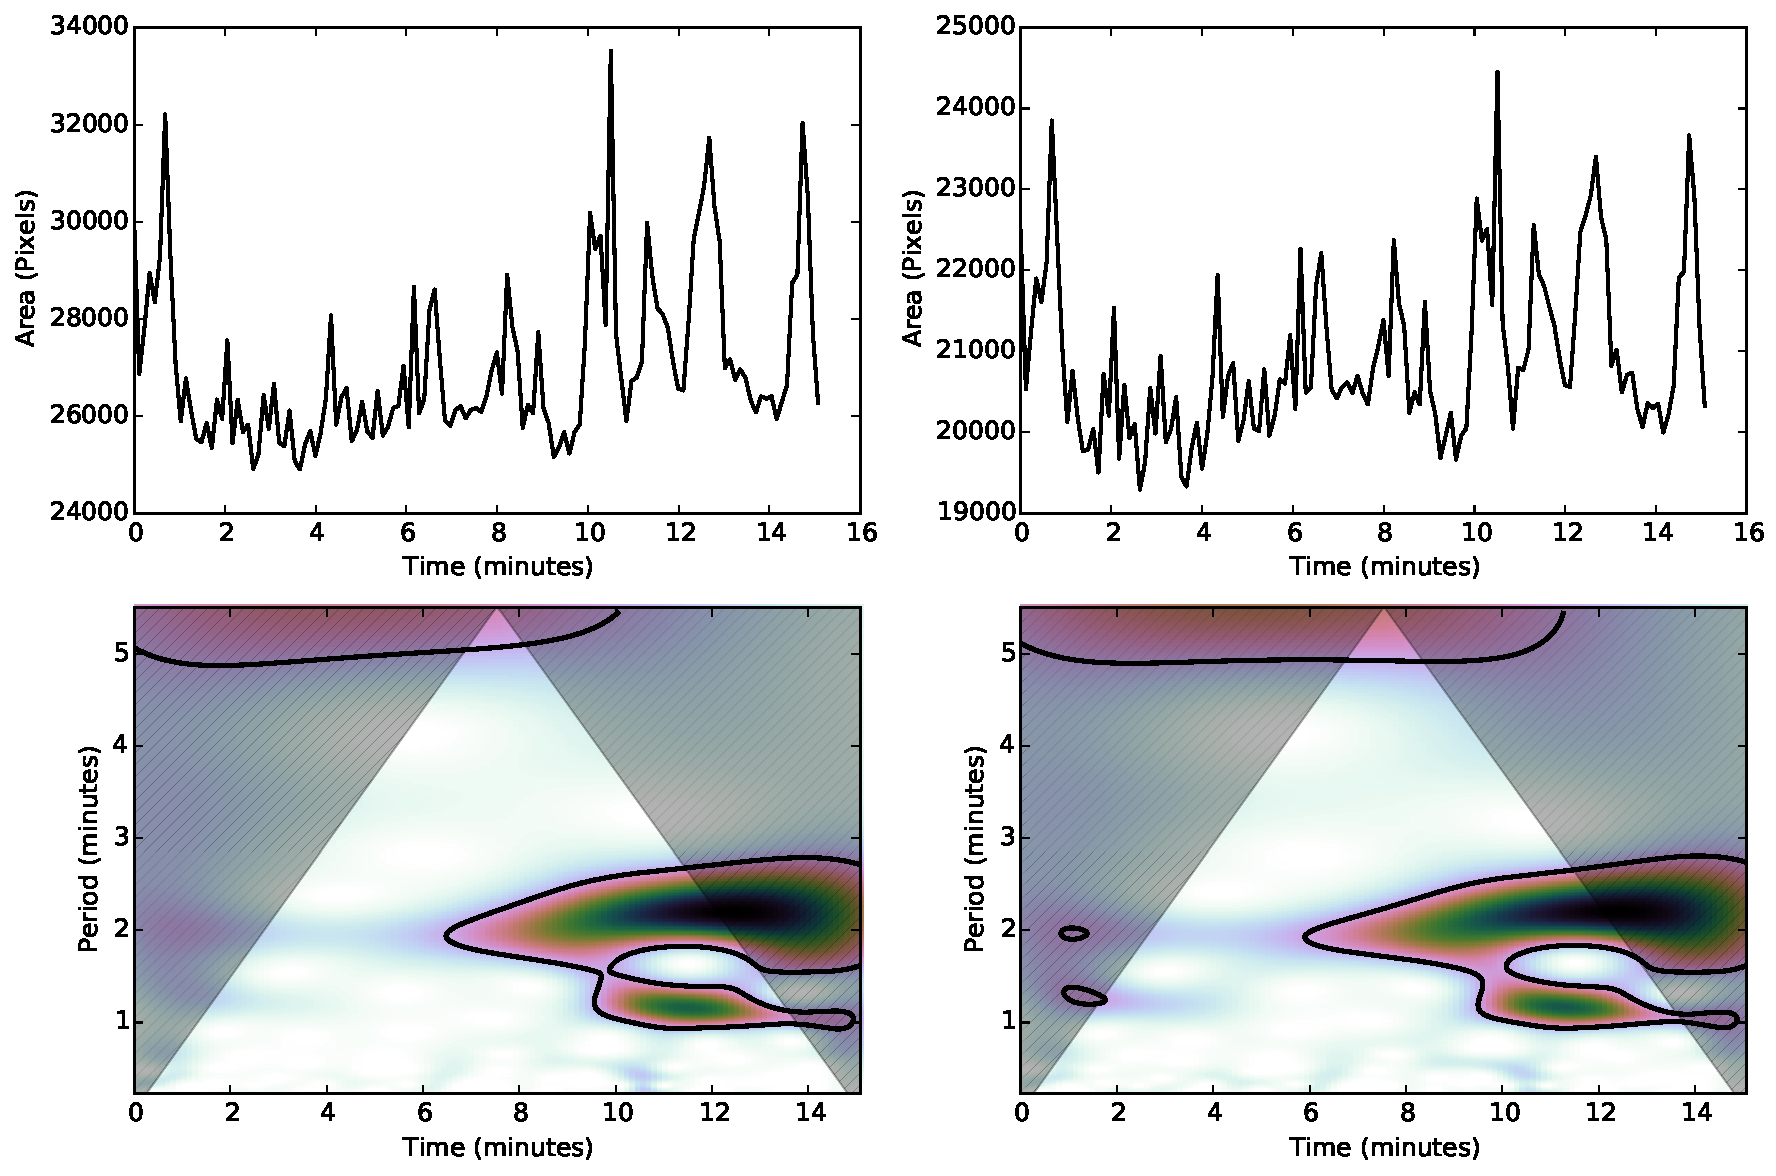
\includegraphics[width=0.75\textwidth]{sunspot_wavelet.pdf}
        \caption{
            The top row shows the cross-sectional area signals returned from a sigma multiplier of 3 and 4.5 for the sunspot observed in IBIS.
            These correspond to the blue and orange contours in Figure \ref{fig:method_overview}.
            The bottom row shows the resultant wavelet transforms of these two signals.
            The cross-hatch region is the cone of influence, while the black contour line is the 95\% significance level.
            The returned wavelet transforms images show that for the IBIS sunspot, the different in sigma multipliers causes no difference in the detected area oscillations.
        }
        \label{fig:sunspot_wavelet}
    \end{sidewaysfigure}
    
    \begin{sidewaysfigure}
        \centering
        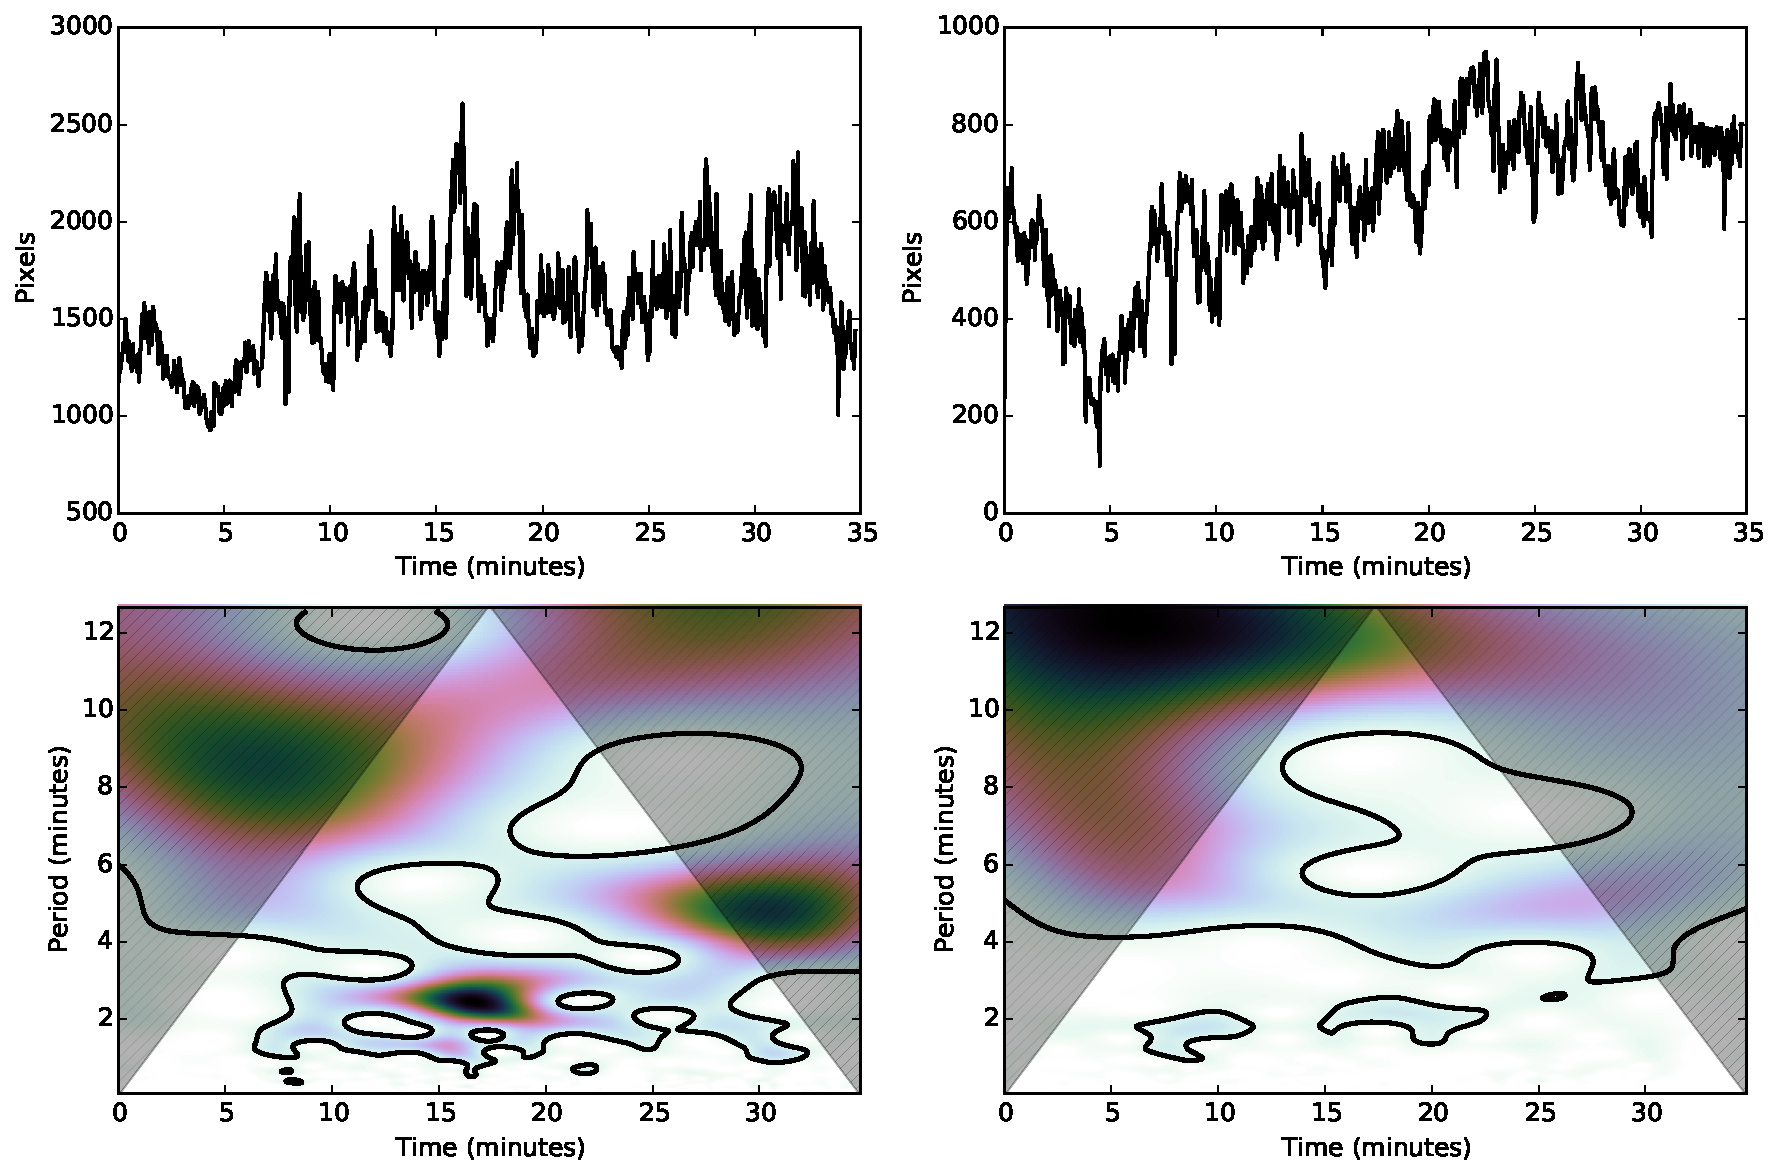
\includegraphics[width=0.75\textwidth]{pore_wavelet.pdf}
        \caption{
            Same as Figure \ref{fig:sunspot_wavelet} but for the magnetic pore observed in ROSA.
            The lowest sigma multiplier is 2 and the largest is 3.5. 
            These correspond to the blue and orange contours in Figure \ref{fig:method_overview}.
            Unlike the sunspot, there is a clear difference between the different sigma multipliers.
            The periods at 2 and 3 minutes are not shown in the largest case and this showcases that for smaller magnetic structures, the sigma multiplier is very important. 
        }
        \label{fig:pore_wavelet}
    \end{sidewaysfigure}
    
    The IBIS sunspot shows little change between the sigma multipliers.
    Since the range of sigma multipliers correspond to the plateau region, the returned cross-sectional area does not catch the penumbra, so the signal that corresponds to either one is focused heavily on the umbra and detects the periods found in the umbra.
    Thus, for this range of sigma multipliers, the same periods are found within this dataset.
    The short length of this data series means that it is impossible to find larger period oscillations, so the only periods found in this sunspot are 1 and 2 minute oscillations.
       
    Now, for the magnetic pore observed in ROSA and with a longer signal.
    The most obvious difference here is the variation of power at periods that are 3 minutes and less for the lower sigma multiplier i.e., 2.
    This power has basically disappeared for the larger multiplier (3.5) but still lingers on.
    The other difference is minor, but it is for the larger periods seen at 5 and 9 minutes.
    While they are under the cone of influence, they are seen clearer and are more powerful for the smaller sigma multiplier.
    However, both multipliers still have the same oscillation periods regardless.
    The cause of this difference would be that the larger multiplier under samples the magnetic pore and this has caused a large difference as expected.
    However, this reveals that the difference here is still small, it would matter most if the wavelet power was used to measure the amplitude of these oscillations.
    Overall, the conclusion for this analysis is that the value of sigma will not vary the result as long as  the range of sigma multipliers is sane.
